\documentclass[10pt,a4paper]{article}
\usepackage[utf8]{inputenc}
\usepackage{amsmath}
\usepackage{amsfonts}
\usepackage{amssymb}
\usepackage{graphicx}
\usepackage[left=2cm,right=2cm,top=2cm,bottom=2cm]{geometry}
\title{Exploring Support Vectors Machines and Least Squares Support Vector Machines}
\author{Boris Shilov}

\begin{document}
\maketitle
\section{Exercise I: Basic support vector machines}
\section{Exercise II: Function estimation and time series prediction}

In this exercise I will attempt to explore the least squares support vector machine formulation using the LS-SVM Matlab toolbox \cite{pelckmansLSSVMlabMATLABToolbox}, particularly function estimation and time series prediction. 

Least-squares support vector machine is an extension of the support vector machine approach in which the quadratic problem of the classic SVM formulation is replaced by the problem of solving a set of linear equations, which is more tractable, giving a large improvement in performance. A drawback presents itself in the fact that LS-SVM requires all of the training points to be used, and hence the solution is no longer sparse, unlike the classic approach where one need only preserve a few support vectors. LS-SVM uses a least squares cost function, as the name implies, but also uses equality constraints, unlike SVM \cite{valyonRobustLSSVMRegression2007}. The function to be minimised over the set of weights $w$, the bias term $b$ and the $e$ error to find a solution in LS-SVM is:
$$
J_p(\mathbf{w}, e) = \frac{1}{2}\mathbf{w}^T\mathbf{w} + C \frac{1}{2} \sum^N_{i=1}{e^2_i}
$$

With equality constraints $d_i = \mathbf{w}^T\varphi(\mathbf{x_i}) + b + e_i$, where $\varphi$ is some function that maps $\mathbf{x_i}$ into a higher dimensional feature space.

We can vary $e$ and also the $C$ penalty parameter, increasing which places more weight on $e$ variables.

\subsection{Support vector machine for function estimation}
Using the \texttt{uiregress} graphical command, we can construct toy datasets. 

First, let us create a dataset where a linear classifier is optimal. One such example is a close cloud of points that are intended to have come from a straight line, which we construct to have 43 points. Increasing $e$ above $0.25$ leaves no support vectors, under the number of support vectors goes up to the number of training points, when $C$ is held fixed at infinity. Decreasing $C$ leads the line to align with the principal direction of the cloud. Setting $C=0.5$ and $e=0.1$ leads to a good fit. Noticeably, the sparsity property comes into play here. By setting the $e$ parameter above zero, we ignore errors smaller than this value. Hence, we only use a subset of the training points, achieving a measure of sparseness. This is similar to the $\epsilon$-insensitive loss function in standard SVM \cite{valyonRobustLSSVMRegression2007}.

\begin{figure}[h]
  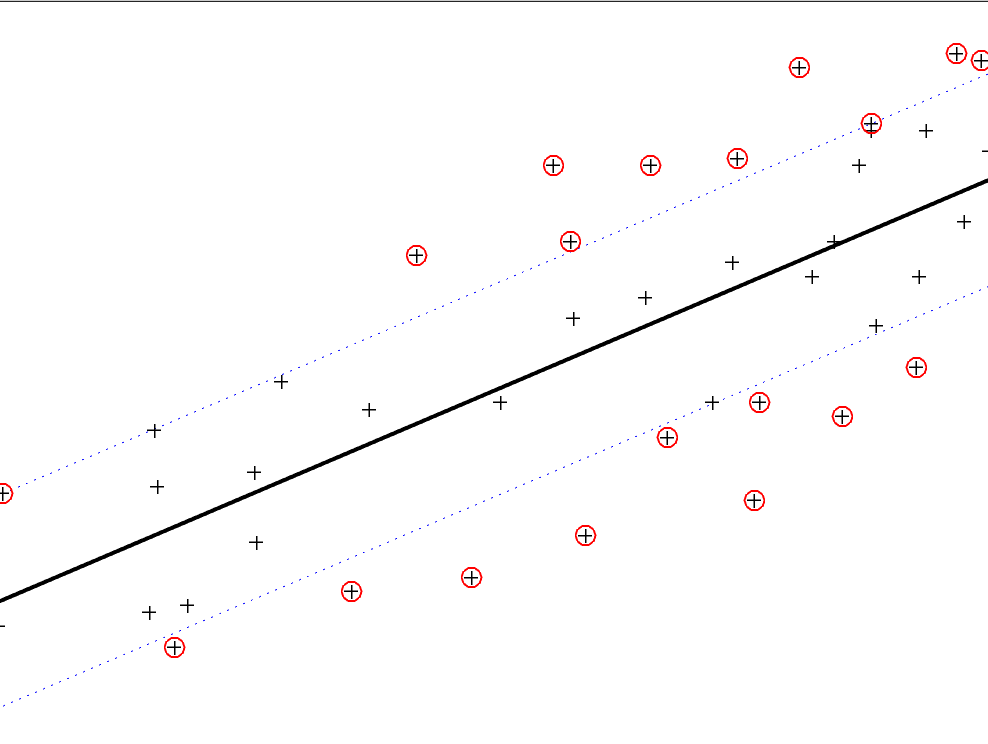
\includegraphics[width=3in]{uiregressFinal.png}
  \caption{A linear least squares classifier fitted to a data cloud of 43 points with parameters $C=0.5$ and $e=0.1$. Given these parameters, only 23 points are used as support vectors, labelled in red.}
  \label{fig:uiregress}
\end{figure}

\subsection{Sinc function}
We can construct an example dataset using a noisy sinc function. Sinc is thus the true data generating process, and the task of an LS-SVM classifier will be to approximate this function without overfitting to replicate the noise.x

We can attempt approximation using the RBF kernel, iterating over a small parameter space.

It seems that the fifth and sixth models are the best fitting on training set. Their parameters are:

We can choose between them, as well as the first two models which are relatively well fitting, using the AUC of test set performance.

It seems the fifth model fits the best on the test case. We may visualise the fifth model on the test data points. Here the hollow points are the test set that was not used to fit the data.


\subsection{Automatic Relevance Determination}

\subsection{Robust regression}
\bibliographystyle{acm}
\bibliography{SVMbib}
\end{document}